\documentclass[11pt]{article}
\usepackage[a4paper,margin=1in]{geometry}
\usepackage{amsmath,amssymb,amsfonts,mathtools}
\usepackage{graphicx}
\usepackage{booktabs}
\usepackage{enumitem}
\usepackage{lineno}
\usepackage[hidelinks]{hyperref}
\usepackage{authblk}
\setlength{\parskip}{0.3em}
\newcommand{\Om}{\Omega}
\newcommand{\eps}{\varepsilon}

\title{\textbf{Coupled Dispersion characteristics of a Flexible Plate
Waveguide with Low-Mach Poiseuille flow}}
\author[1]{Ashray Saxena}
\affil[1]{\small Department of Mechanical Engineering, Birla Institute of Technology \& Science Pilani, Pilani Campus, India}
\date{\today}

\begin{document}
\maketitle

\begin{abstract}
\noindent
The question addressed in this paper is how the free wavenumbers of a two-dimensional
structural--acoustic waveguide change when the fluid column is bounded not by a single flexible plate
facing a rigid wall but by two flexible plates, and how they change again once that fluid is set in
motion by a mean Poiseuille flow. Throughout, the fluid-loading parameter $\eps=\rho a/m$ is treated as the small
quantity of an asymptotic expansion. We first obtain the coupled dispersion relation in closed form and
show that, for identical plates, it factorises exactly into independent symmetric and antisymmetric
families, with the familiar single-plate relation recovered in the rigid-wall limit. Building on this,
a complete first-order catalogue of the coupled wavenumbers is assembled for both families. It covers
the structural, plane-wave and cut-on branches together with the local $\sqrt{\eps}$ expansions that
become necessary wherever two branches would otherwise cross, and every closed-form expression is
checked against the exact numerical roots. One consequence stands out: the single rigid-duct cut-on
ladder of the one-plate problem splits into interleaved even and odd ladders that exchange parity as the
fluid loading grows, so that each branch migrates from a rigid-walled to a pressure-release wavenumber.
The column is then allowed to carry a Poiseuille mean flow. The pressure perturbation now satisfies the
Pridmore--Brown equation with plate-admittance boundary conditions, and a Fredholm solvability argument
gives a closed-form $O(M)$ correction to every coupled wavenumber, which is carried to $O(M^2)$ and
separated into distinct convection and shear contributions. A critical layer appears once the axial
phase Mach number reaches unity, that is at $M_{\rm crit}=\Om/\xi\approx\sqrt{\Om}$, and hence only for
the subsonic structural wave below coincidence. Its inviscid (Frobenius) structure, causal
continuation, and viscous regularisation are analysed; the inner layer has the classical thickness
$Re^{-1/3}$ and the phase jump $-\mathrm{i}\pi$. Solving the viscous linearised Navier--Stokes problem
above $M_{\rm crit}$ shows that the eigenvalue stays regular there and that the discrete wall modes are
not absorbed by the critical layer: their decay is controlled by the wall Stokes layers, scales as
$Re^{-1/2}$, and disappears in the inviscid limit. Every analytical result is corroborated by three
independent numerical methods, namely Runge--Kutta shooting, Chebyshev spectral collocation, and a
primitive-variable formulation reduced symbolically to Pridmore--Brown form, which agree with one
another to about one part in $10^{9}$.
\\[1ex]
\noindent\textbf{Keywords:} structural acoustics; fluid--structure coupling; dispersion relation;
asymptotic analysis; Pridmore--Brown equation; critical layer.
\end{abstract}

\section*{Nomenclature}
\noindent\begin{tabular}{@{}l@{\hspace{1em}}p{0.55\textwidth}@{}}
$a$ & fluid-column height (plate separation)\\
$c,\ \rho$ & sound speed, fluid density\\
$D_j=E_jI_j$ & flexural rigidity of plate $j$ ($I_j=h_j^3/[12(1-\nu_j^2)]$)\\
$E_j,\ \nu_j,\ h_j,\ \rho_{p,j}$ & Young's modulus, Poisson ratio, thickness, density of plate $j$\\
$G_j=D_jk_x^4-m_j\omega^2$ & in-vacuo plate (bending) operator\\
$f(\eta)=4\eta(1-\eta)$ & normalised Poiseuille velocity profile\\
$k=\omega/c$ & acoustic wavenumber\\
$k_x,\ k_y=\sqrt{k^2-k_x^2}$ & axial and transverse wavenumbers\\
$k_c,\ \omega_c$ & coincidence wavenumber and frequency of plate~1\\
$l=k_ca$ & non-dimensional gap\\
$m_j=\rho_{p,j}h_j$ & mass per unit area of plate $j$\\
$M=U_0/c$ & centreline Mach number\\
$p,\ \hat p=p/\rho c^2$ & acoustic pressure perturbation (dimensional, non-dimensional)\\
$Re=ca/\nu$ & acoustic Reynolds number ($\nu$ = kinematic viscosity)\\
$r_D=D_2/D_1,\ r_m=m_2/m_1$ & plate stiffness and mass ratios\\
$S_1=\xi^4/\Omega^2-1,\ S_2=r_D\xi^4/\Omega^2-r_m$ & scaled plate operators\\
$U(y)=U_0f,\ U_0$ & mean flow and its centreline maximum\\
$u,v\ (\hat u,\hat v)$ & axial, transverse velocity perturbations (non-dimensional)\\
$w_j$ & transverse displacement of plate $j$\\
$x,\ y\ (\eta=y/a)$ & axial and transverse coordinates\\
$\alpha_j=k_yG_j/\omega^2\rho$ & plate fluid-loading admittance\\
$\beta_j=\varepsilon/(l^2\Omega^2S_j)$ & viscous plate-admittance (Robin) coefficient\\
$\varepsilon=\rho a/m_1$ & fluid-loading parameter\\
$\eta_c$ & critical-layer location ($\hat\sigma(\eta_c)=0$)\\
$\delta\sim Re^{-1/3}$ & viscous critical-layer thickness\\
$\xi=k_x/k_c$ & non-dimensional axial wavenumber (eigenvalue)\\
$\sigma=\omega-k_xU,\ \hat\sigma=\Omega-M\xi f$ & Doppler-shifted frequency (dimensional, non-dimensional)\\
$\tau=k_ya=l\sqrt{\Omega^2-\xi^2}$ & non-dimensional transverse wavenumber\\
$\Omega=\omega/\omega_c$ & non-dimensional frequency\\
$M_{\rm crit}=\Omega/\xi$ & critical-layer onset Mach number\\
\end{tabular}\\[0.5ex]
\noindent\emph{Subscripts/superscripts:} $1,2$ -- plate~1, plate~2; $s,a$ -- symmetric, antisymmetric
family; $c$ -- coincidence or critical layer; $0$ -- leading ($M=0$ or $\varepsilon=0$) value.

\section{Introduction}
One of the basic questions in structural acoustics is what happens to a wave once a structure and a
fluid are allowed to interact: how the bending wavenumber of a structure vibrating in vacuo is shifted
when the structure is placed in contact with a fluid, and, conversely, how an acoustic wavenumber is
shifted by the presence of a flexible boundary. When the fluid is \emph{enclosed} by flexible walls the
behaviour is quite different from that of an unbounded fluid. There are no branch cuts to contend with,
but instead a sequence of cut-on phenomena appears, each transverse mode beginning to propagate above
its own threshold frequency~\cite{fahy,morseingard}. The simplest bounded configuration of this kind is
a fluid layer held between two identical flexible plates. Fahy~\cite{fahy} analysed it for the symmetric
modes alone and obtained dispersion curves numerically, but those curves could not easily be traced
back to the uncoupled structural and acoustic waves from which they originate.

The step that made such tracing possible was taken by Sarkar and Sonti~\cite{sarkarsonti} for the
closely related waveguide consisting of one flexible plate facing a rigid cover plate. Their idea was to
write the coupled dispersion relation as the in-vacuo structural relation plus a correction produced by
the fluid, and then to expand the coupled wavenumbers as a power series in a fluid-loading parameter
$\eps=\rho a/m$, the ratio of the mass of the fluid column to the mass per unit area of the plate. When
$\eps$ is set to zero the uncoupled wavenumbers are recovered exactly, and the first-order term then
follows each coupled branch continuously away from its uncoupled parent. This makes the physics
transparent: the fluid loading is seen to act in turn like an added mass and like an added stiffness,
and wherever two uncoupled curves would have intersected the coupling instead opens a small gap. The
method rests on the older asymptotic treatment of fluid loading by Morse and Ingard~\cite{morseingard}
and Crighton~\cite{crighton}, but is adapted to a bounded fluid in which the cut-ons, rather than branch
cuts, govern the behaviour.

The same group developed this asymptotic-tracking framework considerably further. Sarkar, Kunte and
Sonti~\cite{kunte2011} showed that flexible structural-acoustic waveguides of quite different
cross-sections (rectangular, circular-cylindrical and elliptical) all obey a single generic form of the
dispersion relation, so that their coupled-wavenumber solutions can be drawn on one common schematic,
and Prakash and Sonti~\cite{prakash2016} carried the catalogue over to arbitrary fluid loading rather
than only small or large $\eps$. It is important to be clear that all of this work concerns a
\emph{quiescent} fluid. The two-flexible-plate symmetric and antisymmetric catalogue worked out in
Sections~2 and~3 below is therefore best regarded as a special case that reproduces and tidies up these
known quiescent results, and it is presented here mainly for completeness and as the $M=0$ baseline for
what follows. The genuinely new ingredient is the mean flow. In a wide range of situations, from
compliant ducts to physiological flow in elastic vessels and to flow-induced sound more
generally~\cite{morab}, the fluid is not at rest, and the mean flow couples the structural and acoustic
waves through both convection and shear. It also raises the possibility of a \emph{critical layer},
a location at which the axial phase speed of the wave equals the local speed of the flow. Acoustics in a
sheared mean flow is governed by the Pridmore--Brown equation~\cite{pridmorebrown}, and although the
critical-layer singularity and its viscous resolution have been studied at length for lined
ducts~\cite{brambley,brambleydarau,maslowe}, they do not appear to have been examined for the
two-flexible-plate waveguide.

Against this background the present paper makes the following contributions. The coupled dispersion
relation for two flexible plates is derived in closed form, its exact symmetric/antisymmetric
factorisation is established, and the single fluid-loaded-plate dispersion relation is recovered as a
limit. The first-order
asymptotic catalogue is then assembled for both symmetry families, including the local $\sqrt{\eps}$
windows around coincidence and the cut-ons, and is checked numerically. A Poiseuille mean flow is
introduced next, and a closed-form $O(M)$ correction, together with the $O(M^2)$ correction and its
convection/shear split, is obtained for every coupled wavenumber. Finally the critical-layer threshold
$M_{\rm crit}=\Om/\xi$ is established and the inviscid and viscous structure of the layer is analysed,
with all results confirmed by three independent numerical methods. The first two of these contributions
reproduce and organise, for the two-plate geometry, results that are consistent with the quiescent
framework of~\cite{sarkarsonti,kunte2011,prakash2016}; the new material is the treatment of the mean
flow. It should also be said plainly that sheared-flow duct acoustics and its critical layer are well
established in their own right~\cite{pridmorebrown,brambleydarau,maslowe}; what is new here is the
combination of that machinery with the flexible-plate asymptotic-tracking framework, and the closed-form
low-Mach corrections and wall-mode conclusions that follow from it, rather than the critical-layer
phenomenology itself.

\section{Formulation and coupled dispersion relation}
Consider a two-dimensional acoustic fluid of density $\rho$ and sound speed $c$ occupying the strip
$0\le y\le a$ and unbounded in $x$, with every field taken to be independent of $z$ and a time
dependence $e^{i\omega t}$ understood and suppressed. Thin elastic plates close the strip at $y=0$
(plate~1) and $y=a$ (plate~2); each has flexural rigidity $D_j=E_jI_j$ with
$I_j=h_j^3/[12(1-\nu_j^2)]$, and mass per unit area $m_j=\rho_{p,j}h_j$. The acoustic pressure is written
as the sum of two transverse-travelling components,
$p=(A e^{-ik_yy}+Be^{ik_yy})e^{-ik_xx}$ with $k_x^2+k_y^2=k^2=\omega^2/c^2$, and the transverse particle
velocity follows from the linearised Euler relation. Requiring the normal velocity to match the plate
velocity at each wall, $v=i\omega w_j$, and imposing the plate equations $G_jw_j=\mp p$ with
$G_j=D_jk_x^4-m_j\omega^2$, closes the problem. Eliminating the two amplitudes $A$ and $B$ and writing
$\alpha_j\equiv k_yG_j/\omega^2\rho$ for the dimensionless admittance of each plate gives the coupled
dispersion relation,
\begin{equation}
(1+i\alpha_1)(1+i\alpha_2)=e^{2ik_ya}(1-i\alpha_1)(1-i\alpha_2)
\ \Longleftrightarrow\
\tan(k_ya)=\frac{\alpha_1+\alpha_2}{1-\alpha_1\alpha_2}.
\label{eq:disp}
\end{equation}
Two checks confirm that \eqref{eq:disp} is the right object. Letting the second plate become rigid,
$\alpha_2\to\infty$, reduces it to $\alpha_1=-\cot(k_ya)$, that is to
$D_1k_x^4-m_1\omega^2=-(\omega^2\rho/k_y)\cot(k_ya)$, which is the classical dispersion relation for a
single fluid-loaded plate backed by a rigid wall~\cite{sarkarsonti}. When
the two plates are identical the relation factorises cleanly into two independent problems,
\begin{equation}
\text{(symmetric, $v{=}0$ at $y{=}a/2$)}\ \alpha=-\cot\tfrac{k_ya}{2},
\qquad
\text{(antisymmetric, $p{=}0$ at $y{=}a/2$)}\ \alpha=+\tan\tfrac{k_ya}{2}.
\end{equation}
The symmetric branch is simply the single-plate problem with $a$ replaced by $a/2$, equivalent to a
flexible plate over a rigid wall placed at the mid-plane~\cite{fahy}. Non-dimensionalising on the coincidence condition of plate~1, with
$\Om=\omega/\omega_c$, $\xi=k_x/k_c$, $l=k_ca$, $\tau=k_ya=l\sqrt{\Om^2-\xi^2}$ and
$S_1=\xi^4/\Om^2-1$, the two families take the compact form
\begin{equation}
\text{(SYM)}\ \Big(\tfrac{\xi^4}{\Om^2}-1\Big)\tau\tan\tfrac{\tau}{2}+\eps=0,
\qquad
\text{(ANTI)}\ \Big(\tfrac{\xi^4}{\Om^2}-1\Big)\tau\cot\tfrac{\tau}{2}-\eps=0.
\label{eq:nd}
\end{equation}
Setting $\eps=0$ exposes the uncoupled parents from which the coupled branches grow: the structural wave
$\xi=\Om^{1/2}$, which belongs to both families, the plane wave $\xi=\Om$ and the even cut-ons
$\tau=2n\pi$, which are symmetric, and the odd cut-ons $\tau=(2n{+}1)\pi$, which are antisymmetric and,
notably, have no plane-wave member.

\section{Asymptotic catalogue ($\eps\ll1$ and $\eps\gg1$)}
Each parent wavenumber can be followed into the coupled problem by writing it as the uncoupled value
plus a correction, for instance $\xi=\Om^{1/2}+a_1\eps$, and balancing the powers of $\eps$ that result.
Carrying this out for the structural wave gives, with $\tau_s=l\sqrt{\Om^2-\Om}$,
\begin{equation}
\xi_s^{\rm sym}=\Om^{1/2}-\frac{\eps}{4l\sqrt{\Om-1}\,\tan(\tau_s/2)},\qquad
\xi_s^{\rm anti}=\Om^{1/2}+\frac{\eps\tan(\tau_s/2)}{4l\sqrt{\Om-1}},
\end{equation}
while the symmetric plane wave becomes $\xi_a=\Om+\eps/[\Om l^2(\Om^2-1)]$ and the cut-on branches of
both families take the common form $\xi_a^{(m)}=\sqrt{\Om^2-(m\pi/l)^2}+2\eps/(S_0l^2\xi_0)$ with $m$
even for the symmetric family and odd for the antisymmetric one. This regular expansion fails close to
coincidence and close to each cut-on, where two parents approach one another and the correction grows
without bound; there a local rescaling in $\sqrt{\eps}$ is required instead. It produces gaps of the
form $\xi=\Om\pm\sqrt{\eps}/(2l)$ at the symmetric coincidence and $\xi=\sqrt{\Om_c}\pm\sqrt{2\eps}/(2l)$
at the cut-on crossings of both families, and it shows that the antisymmetric structural wave passes
through coincidence without a gap, its correction remaining finite with $a_1\to\tfrac18$. In the
opposite limit of heavy fluid loading, $\eps\gg1$, the parents are no longer the rigid-duct cut-ons but
the pressure-release cut-ons, and the parity of the symmetric and antisymmetric ladders is exchanged
relative to the small-$\eps$ case. Each branch therefore drifts steadily from a rigid-walled to a
pressure-release wavenumber as the loading increases, and the two cut-on ladders interleave along the
way. Every one of these closed-form expressions reproduces the exact numerical roots to better than half
a percent within its range of validity, as documented in Section~\ref{sec:val}.

\section{Uniform Poiseuille mean flow}
Suppose now that the column carries a Poiseuille flow, $U(y)=4U_0(y/a)(1-y/a)=U_0f(\eta)$ with
$f=4\eta(1-\eta)$ and $\eta=y/a$, satisfying no-slip at both walls, $U(0)=U(a)=0$, and characterised by
the centreline Mach number $M=U_0/c$. In a sheared mean flow the pressure perturbation no longer obeys
a constant-coefficient equation but the Pridmore--Brown equation, which in the present non-dimensional
variables, with the Doppler-shifted frequency written as $\hat\sigma=\Om-M\xi f$, reads
\begin{equation}
\hat p_{\eta\eta}+\frac{2M\xi f'}{\hat\sigma}\,\hat p_\eta+l^2(\hat\sigma^2-\xi^2)\hat p=0,
\qquad f'=4(1-2\eta).
\label{eq:pb}
\end{equation}
The plates enter through the same admittance as before, now expressed as boundary conditions on the
pressure, $\hat p_\eta(0)+(\eps/S_1)\hat p(0)=0$ and $\hat p_\eta(1)-(\eps/S_2)\hat p(1)=0$. A useful
simplification arises because the Poiseuille profile vanishes at the walls: with $U=0$ there, the
convective (Ingard--Myers) correction that ordinarily complicates a moving-wall condition drops out, so
the boundary conditions keep exactly the quiescent form, and at $M=0$ equation~\eqref{eq:pb} collapses
back onto~\eqref{eq:disp}. The sign of the shear term in~\eqref{eq:pb} is the one point that requires
care, and it is fixed independently by the primitive-variable derivation reported in
Section~\ref{sec:val}.

\subsection{Closed-form $O(M)$ and $O(M^2)$ corrections}
Expanding both the wavenumber and the pressure in the Mach number, $\xi=\xi_0+M\xi_1+M^2\xi_2+\dots$ and
$\hat p=p_0+Mp_1+\dots$, the problem at first order in $M$ inherits the same leading operator
$L_0=\partial_\eta^2+\tau_0^2$ as the quiescent case. Because that operator is self-adjoint, its adjoint
null function is simply $p_0$, and the Fredholm solvability condition can be applied directly to give a
closed-form expression for the first correction,
\begin{equation}
\xi_1=\frac{-\tfrac{2}{\Om}\big(p_0(1)^2+p_0(0)^2\big)+\tfrac{4}{\Om}I_0-l^2\Om I_f}
{\,l^2I_0+\tfrac{2\eps\xi_0^2}{\Om^2}\big(r_Dp_0(1)^2/S_2^2+p_0(0)^2/S_1^2\big)},
\quad I_0\!=\!\!\int_0^1\!\!p_0^2,\ I_f\!=\!\!\int_0^1\!\!f p_0^2 .
\label{eq:xi1}
\end{equation}
The correction is negative on every branch, which says that a downstream flow lowers the axial
wavenumber while an upstream flow raises it, and so the dispersion relation is no longer symmetric under
$k_x\to-k_x$. The plane wave is the most strongly affected because it samples the fast core of the
profile most fully. The second-order coefficient $\xi_2$, which is even in $M$ and therefore the same
for upstream and downstream propagation, is obtained by Richardson extrapolation of the numerical
solution and can be split into a part due to convection and a part due to the shear $U'$. The shear
contribution is far from negligible, reaching roughly a third of $\xi_2$ on the plane-wave branch, so a
uniform (plug-flow) model would predict the second-order term incorrectly and the full parabolic profile
must be retained. Including $\xi_2$ noticeably extends the range of $M$ over which the asymptotic
wavenumber remains accurate.

\subsection{Critical layer: inviscid structure and viscous regularisation}
Equation~\eqref{eq:pb} becomes singular wherever $\hat\sigma(\eta)=0$, that is wherever the axial phase
speed of the wave coincides with the local speed of the flow. Since $f$ attains its maximum at the
centreline, the first such point to appear does so there, and it appears once
\begin{equation}
M\ge M_{\rm crit}=\frac{\Om}{\xi}=c_{\rm ph}\qquad(\text{structural wave: } M_{\rm crit}\approx\sqrt{\Om}).
\end{equation}
A critical layer is therefore reachable at subsonic flow only for the subsonic structural wave below
coincidence, where $\Om<1$; above coincidence the structural wave is supersonic and no critical layer
forms until the flow itself becomes sonic. Examined locally, with
$\hat\sigma\simeq\hat\sigma'_c(\eta-\eta_c)$, equation~\eqref{eq:pb} has a regular singular point whose
Frobenius exponents are $\{0,3\}$. The pressure itself therefore stays bounded, carrying only a weak
$(\eta-\eta_c)^3\ln(\eta-\eta_c)$ term, but the cross-stream velocity $v\propto\hat p'/\hat\sigma$
diverges like $(\eta-\eta_c)^{-1}$. Which branch of the logarithm is selected is decided by causality:
the vanishing-viscosity (Landau) prescription indents the integration contour below $\eta_c$ and so
contributes a phase jump of magnitude $\pi$, that is $-\mathrm{i}\pi$, corresponding to net absorption.
A viscous inner layer of thickness $\delta\sim Re^{-1/3}$, governed by the Airy/Tollmien balance,
regularises the singularity and reproduces this same jump as $Re\to\infty$. For the wall-driven modes
of interest here the pressure remains regular at $\eta_c$, so the critical layer shifts the discrete
wavenumbers only weakly, at higher order, and the strong singular response is carried instead by the
cross-stream velocity field and by the continuous spectrum.

\subsection{Viscous solution above $M_{\rm crit}$}
To decide what happens above $M_{\rm crit}$, where the inviscid operator is singular, the problem is
solved once more with viscosity retained. The linearised compressible Navier--Stokes equations, viscous
in the momentum balance and inviscid in the energy balance, are imposed together with no-slip and the
plate-admittance condition and discretised by Chebyshev collocation, which turns the dispersion problem
into a well-posed nonlinear eigenvalue problem at acoustic Reynolds number $Re=ca/\nu$. The boundary
condition that now acts on the normal velocity, $\hat v(0)-\beta_1\hat v_\eta(0)=0$ with
$\beta_1=\eps/(l^2\Om^2S_1)$, reduces exactly to the inviscid plate-admittance condition as
$Re\to\infty$, as shown in Appendix~\ref{app:bc}. The viscous eigenvalue turns out to be perfectly
regular through and above $M_{\rm crit}$ (Fig.~\ref{fig:viscglobal}a): viscosity smooths the
critical-layer singularity over an inner layer whose thickness scales as $Re^{-1/3}$. Sweeping the
Reynolds number then separates the critical-layer effect from everything else. The modal decay rate
$\operatorname{Im}\xi$ is found to scale as $Re^{-1/2}$ both below and above $M_{\rm crit}$
(Fig.~\ref{fig:viscglobal}b), which identifies it as the damping produced by the wall Stokes layers and
shows that it vanishes in the inviscid limit; fitting the data to $\operatorname{Im}\xi=A\,Re^{-1/2}+B$
leaves a finite, $Re$-independent critical-layer part of only $B\approx-1\times10^{-5}$, indistinguishable
from zero at the precision available (Fig.~\ref{fig:viscglobal}c). The conclusion is that the interior
critical layer does not absorb the discrete wall modes at leading order, consistent with the regularity
of the pressure at $\eta_c$, and that these modes remain neutrally propagating, in the inviscid sense,
even above $M_{\rm crit}$. In this respect they differ from the surface modes over an impedance wall, for
which the critical layer can absorb discrete modes significantly~\cite{brambleydarau}.

\begin{figure}[h]
\centering
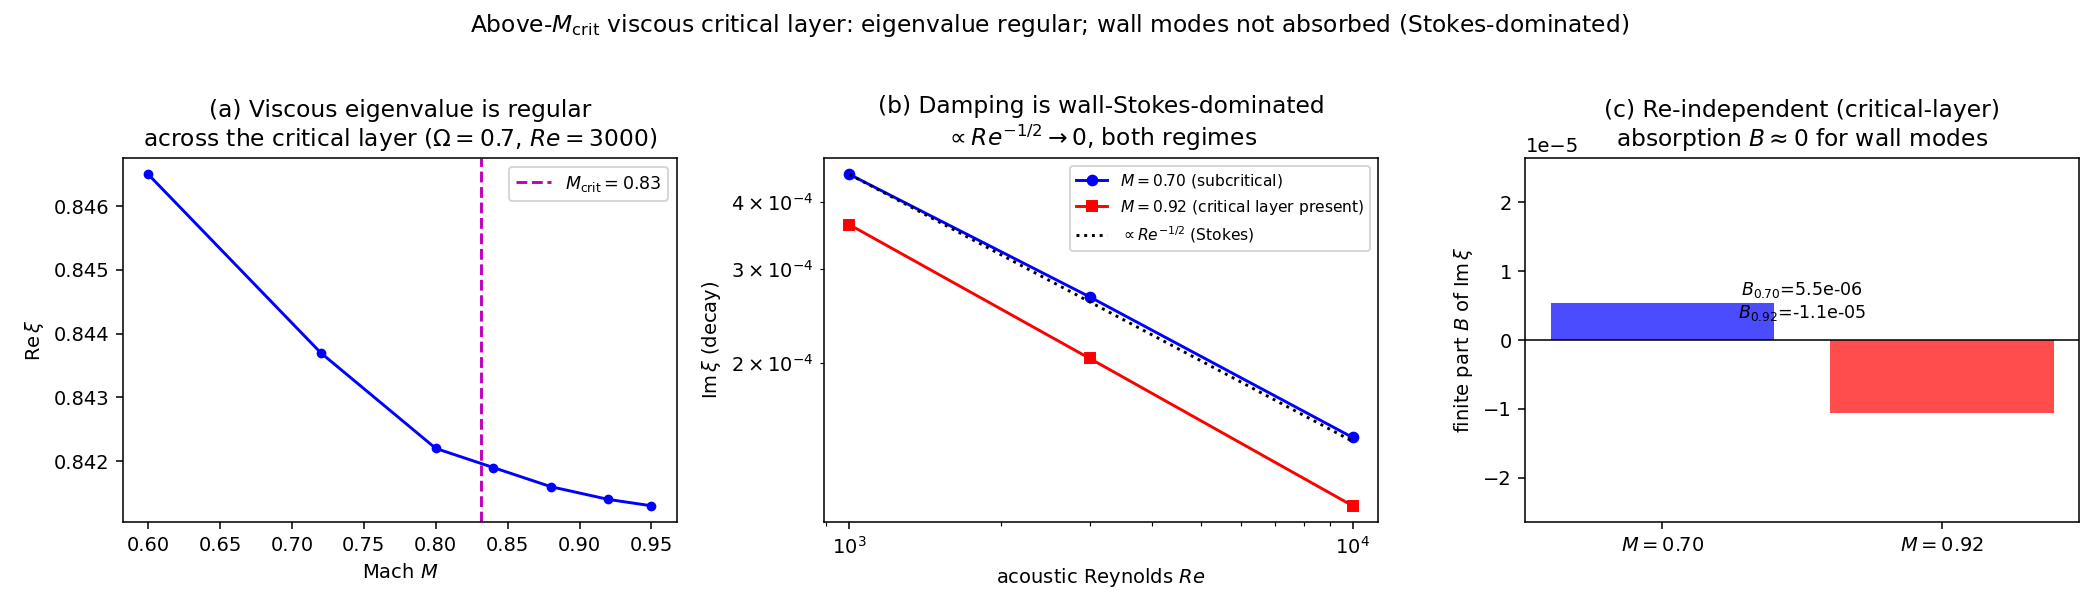
\includegraphics[width=0.98\textwidth]{fig8_viscous_global.png}
\caption{Viscous solution above $M_{\rm crit}$ ($\Om=0.7$). (a) The eigenvalue is regular through the
critical layer ($Re=3000$). (b) The decay rate $\operatorname{Im}\xi\propto Re^{-1/2}$ both below
($M{=}0.70$) and above ($M{=}0.92$) $M_{\rm crit}$, wall-Stokes-dominated and vanishing inviscidly.
(c) The $Re$-independent critical-layer absorption $B\approx0$: the discrete wall modes are not
absorbed by the interior critical layer.}
\label{fig:viscglobal}
\end{figure}

\section{Numerical validation}\label{sec:val}
The analytical results rest on three numerical checks that are independent of one another. The first is
a comparison between a Runge--Kutta shooting integration of~\eqref{eq:pb} and an entirely separate
Chebyshev spectral collocation solution of the same equation; the two agree to about
$6\times10^{-9}$ on every branch for Mach numbers up to $0.2$. The second is that both reduce, at
$M=0$, to the closed-form quiescent relation~\eqref{eq:disp}, whose algebra was itself verified
symbolically. The third is a primitive-variable formulation written in the three fields $u'$, $v'$ and
$p'$ of the linearised Euler equations and reduced symbolically; it returns the Pridmore--Brown
operator~\eqref{eq:pb} exactly, and it was this derivation that fixed the sign of the shear term. As a
direct test of the asymptotics, the closed-form coefficient $\xi_1$ of~\eqref{eq:xi1} agrees with the
numerically differentiated $d\xi/dM$ to within $0.1$--$0.5\%$ (Table~\ref{tab:xi1}), and the symmetric
branch of the quiescent problem reproduces the single fluid-loaded-plate result~\cite{sarkarsonti}
under $(a,\eps)\to(a/2,\eps/2)$ to four decimal places at every frequency.

\begin{table}[h]
\centering
\begin{tabular}{ccccc}
\toprule
$\Om$ & branch ($\xi_0$) & type & $\xi_1$ (closed) & $\xi_1$ (numerical)\\
\midrule
1.3 & 1.1165 & sym structural & $-0.1283$ & $-0.1290$\\
1.3 & 1.1837 & anti structural & $-0.1065$ & $-0.1068$\\
1.3 & 1.3267 & plane wave & $-0.7471$ & $-0.7468$\\
1.8 & 1.8069 & plane wave & $-1.1743$ & $-1.1750$\\
\bottomrule
\end{tabular}
\caption{Closed-form $O(M)$ correction \eqref{eq:xi1} vs.\ numerical $d\xi/dM$ ($l=3$, $\eps=0.25$).}
\label{tab:xi1}
\end{table}

\begin{figure}[h]
\centering
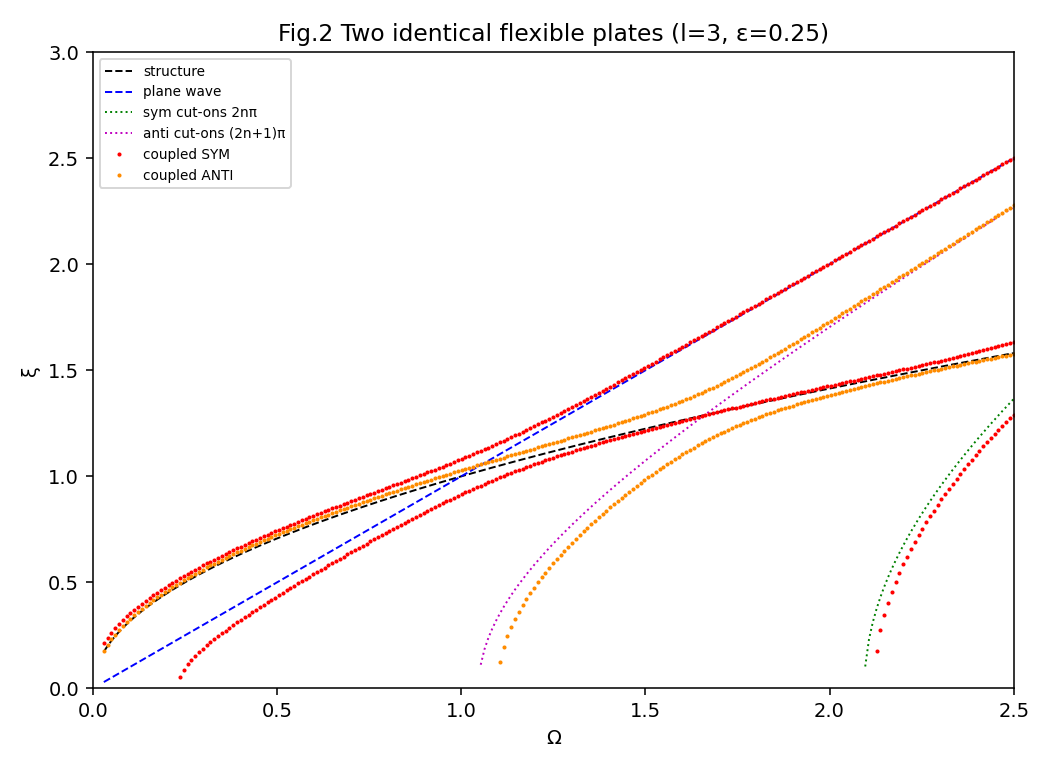
\includegraphics[width=0.9\textwidth]{fig2_two_identical.png}
\caption{Coupled symmetric and antisymmetric dispersion branches for two identical flexible plates
($l=3$, $\eps=0.25$), overlaid on the uncoupled parents. The symmetric family tracks the plane wave
and even cut-ons, the antisymmetric family the odd cut-ons; both perturb the common structural wave
and open gaps at every intersection.}
\label{fig:branches}
\end{figure}

\begin{figure}[h]
\centering
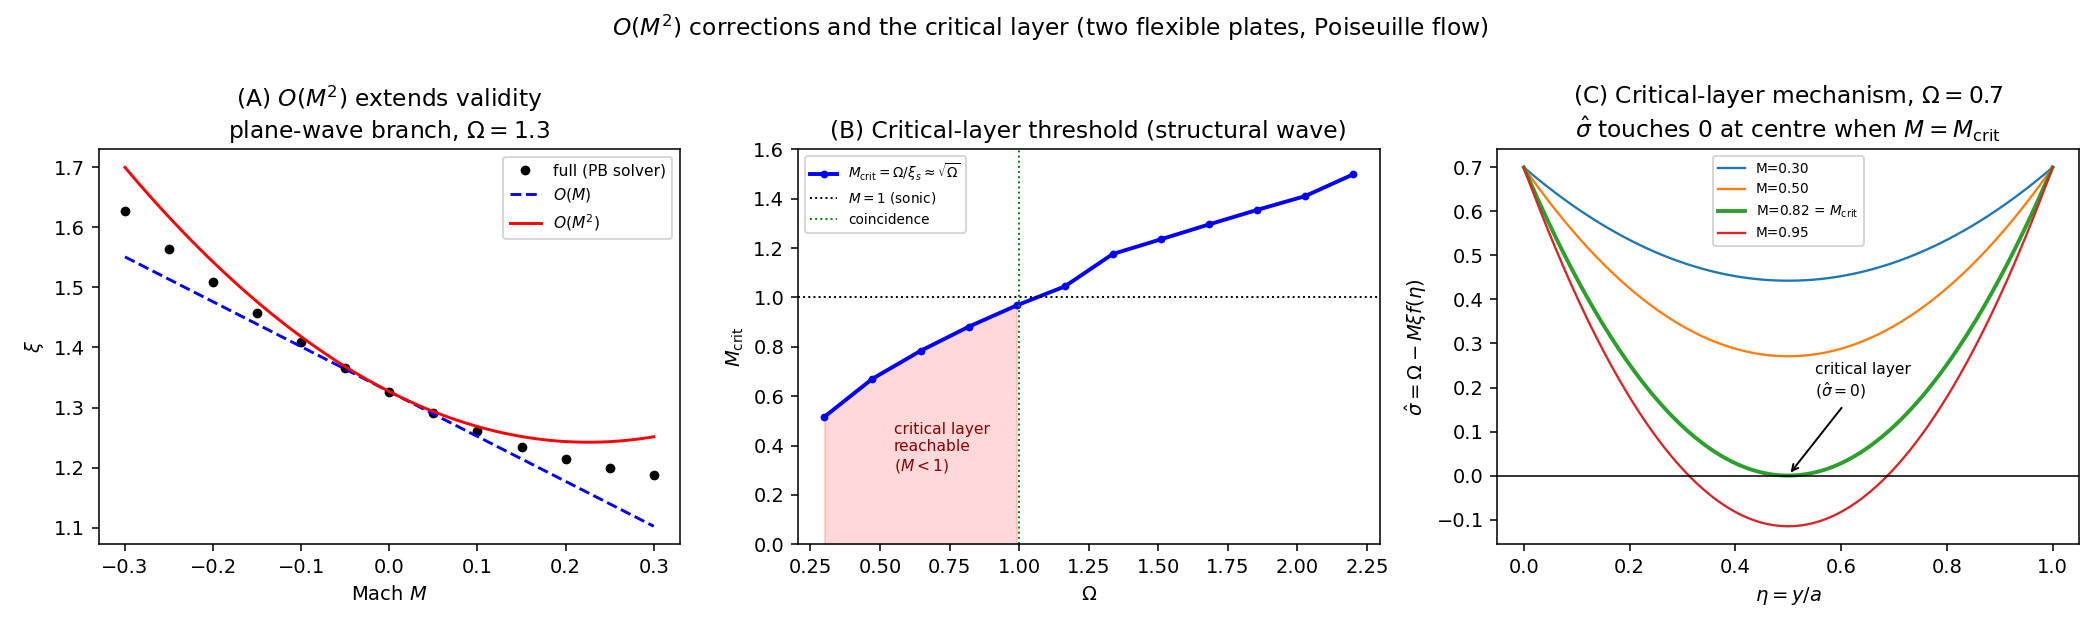
\includegraphics[width=0.98\textwidth]{fig6_om2_critical.png}
\caption{Mean-flow effects. (a) $O(M^2)$ extends the validity of the asymptotic wavenumber beyond
$O(M)$. (b) Critical-layer threshold $M_{\rm crit}=\Om/\xi_s\approx\sqrt{\Om}$ (reachable at subsonic
$M$ only below coincidence). (c) The Doppler-shifted frequency $\hat\sigma(\eta)$ touches zero at the
centreline when $M=M_{\rm crit}$.}
\label{fig:meanflow}
\end{figure}

\begin{figure}[h]
\centering
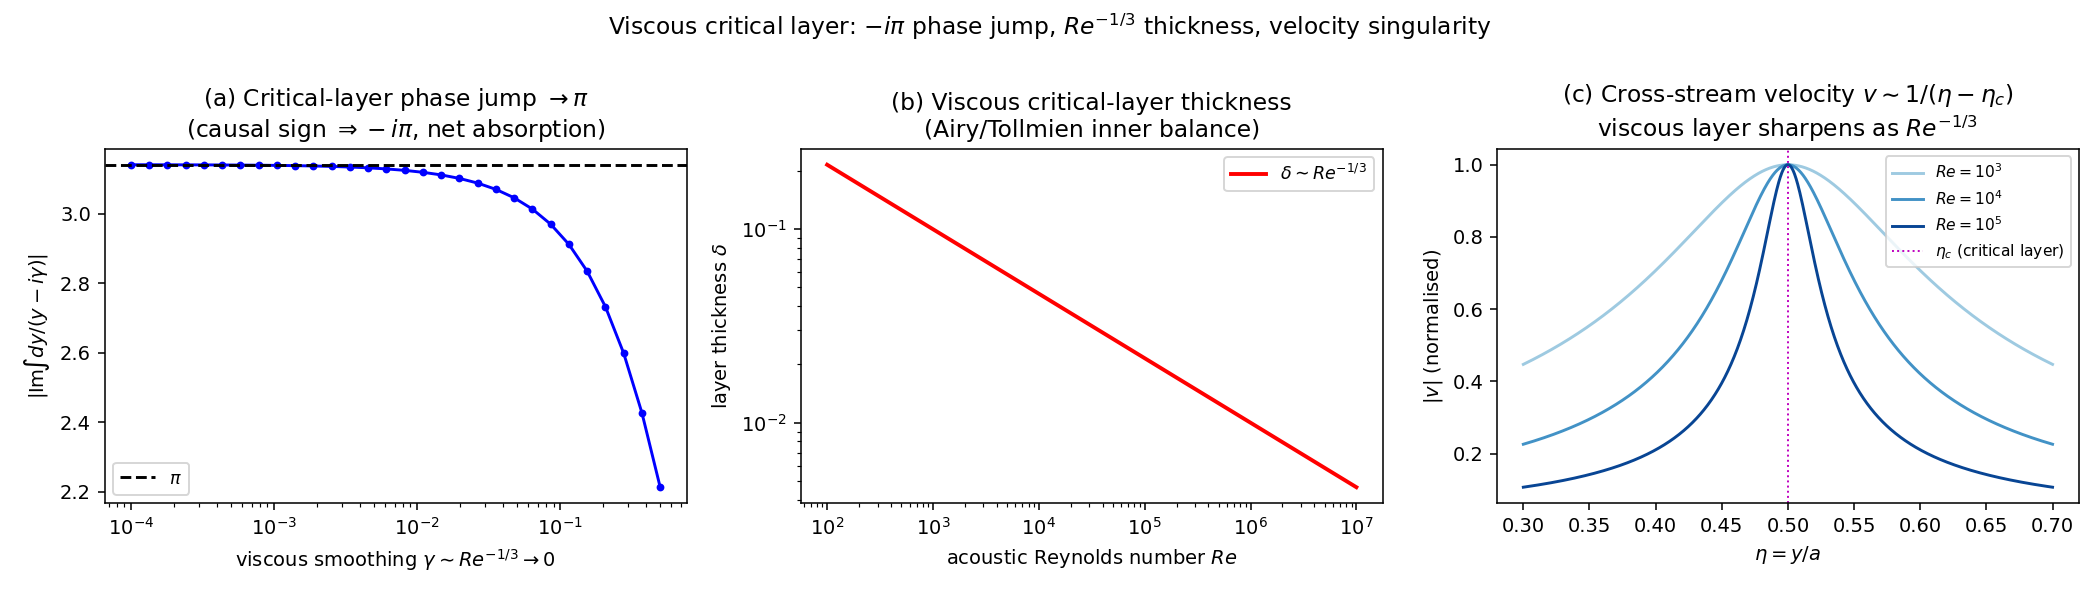
\includegraphics[width=0.98\textwidth]{fig7_viscous_cl.png}
\caption{Viscous critical layer. (a) The causal phase jump tends to $\pi$ in magnitude as the viscous
smoothing vanishes ($-\mathrm{i}\pi$, net absorption). (b) Inner-layer thickness $\delta\sim Re^{-1/3}$.
(c) The cross-stream velocity singularity $v\sim(\eta-\eta_c)^{-1}$, regularised over a layer that
sharpens as $Re^{-1/3}$.}
\label{fig:viscous}
\end{figure}

\section{Results and discussion}
Taken together, the results show that the two-flexible-plate waveguide reduces correctly to every known
limit while adding behaviour that the one-plate problem does not possess. The most visible change is in
the cut-on spectrum, which is now twice as dense as before and is organised into two interleaved
ladders, the even one belonging to the symmetric family and the odd one to the antisymmetric family.
Only the symmetric family inherits the plane wave and, with it, the gap at coincidence; the
antisymmetric structural wave, having no plane wave to collide with, passes straight through coincidence
(Fig.~\ref{fig:branches}). When the two plates are not identical the symmetry decoupling is lost, and
the two structural waves, which would otherwise cross, instead veer away from one another with a minimum
separation $\Delta\xi=\eps/[2l\sqrt{\Om-1}\sin\tau_s]$ at $r_D=r_m=1$ that grows linearly with the fluid
loading. Adding a structural loss factor makes the wavenumbers complex, with the structural branches
attenuating the most and the plane wave the least.

The mean flow shifts every branch at first order in $M$ and adds an even, direction-independent
correction at second order in which, as noted above, the shear plays a substantial part
(Fig.~\ref{fig:meanflow}). The critical-layer threshold separates a regular subsonic-flow regime, in
which the low-Mach asymptotics developed here apply, from a singular regime beyond it. Within the
singular regime the viscous resolution of the layer follows the classical $Re^{-1/3}$ inner structure,
but with one qualification that is specific to this problem: the wall-driven discrete modes couple to
the interior critical layer only weakly. The viscous linearised Navier--Stokes solution
(Fig.~\ref{fig:viscglobal}) confirms that the eigenvalue remains regular through and above
$M_{\rm crit}$, that its decay rate is set by the wall Stokes layers and scales as $Re^{-1/2}$, and that
the $Re$-independent critical-layer absorption is effectively zero. The strong, genuinely singular part
of the critical-layer response therefore lives in the cross-stream velocity field and in the continuous
spectrum rather than in the discrete wavenumbers that are the subject of this paper.

\section{Larger Mach numbers: full dispersion, validity and stability}
The corrections of Section~4.1 are asymptotic in $M$, and to see what happens at larger Mach numbers the
full nonlinear dispersion must be read off directly from~\eqref{eq:pb}. Figure~\ref{fig:Mmap} does this
for $M=0$, $0.3$ and $0.5$ and shows that an increasing downstream flow pushes the whole diagram towards
lower $\xi$, in agreement with the negative sign of $\xi_1$; the shift is largest for the plane-wave-like
branch and smallest for the structural branches, and the cut-on ladder structure survives intact. One
limitation should be stated frankly. A strictly parabolic Poiseuille profile is an idealisation valid at
low Mach number, so the model is quantitative only up to centreline Mach numbers in the transonic range,
and the high-$M$ results are offered as an extension of the model rather than as a prediction for a genuinely
compressible mean flow.

How far the closed-form corrections themselves can be trusted depends strongly on the branch
(Fig.~\ref{fig:valid}a,b). On the flow-sensitive plane-wave branch the $O(M)$ and $O(M^2)$ expansions
pass the five-percent error mark already by $M\approx0.25$--$0.3$, and, being asymptotic rather than
convergent, the series ultimately diverges; on a flow-insensitive structural branch the same expansions
stay accurate to within about three percent out to much larger $M$. The practical message is that the
closed forms are quantitative at low Mach number and that the full solver should be used beyond
$M\sim0.3$ on the sensitive branches. Finally, the convective stability of the system was checked by
computing the complex wavenumber with the viscous solver. The inviscid eigenvalues remain real and the
viscous decay rate satisfies $\operatorname{Im}\xi>0$ throughout the range studied
(Fig.~\ref{fig:valid}c), so the mean flow does not destabilise the structural-acoustic wall modes and no
flow-induced flutter is found up to the transonic limit of the model; the damping that is present comes
from the wall Stokes layers and vanishes as the viscosity is removed.

\begin{figure}[h]
\centering
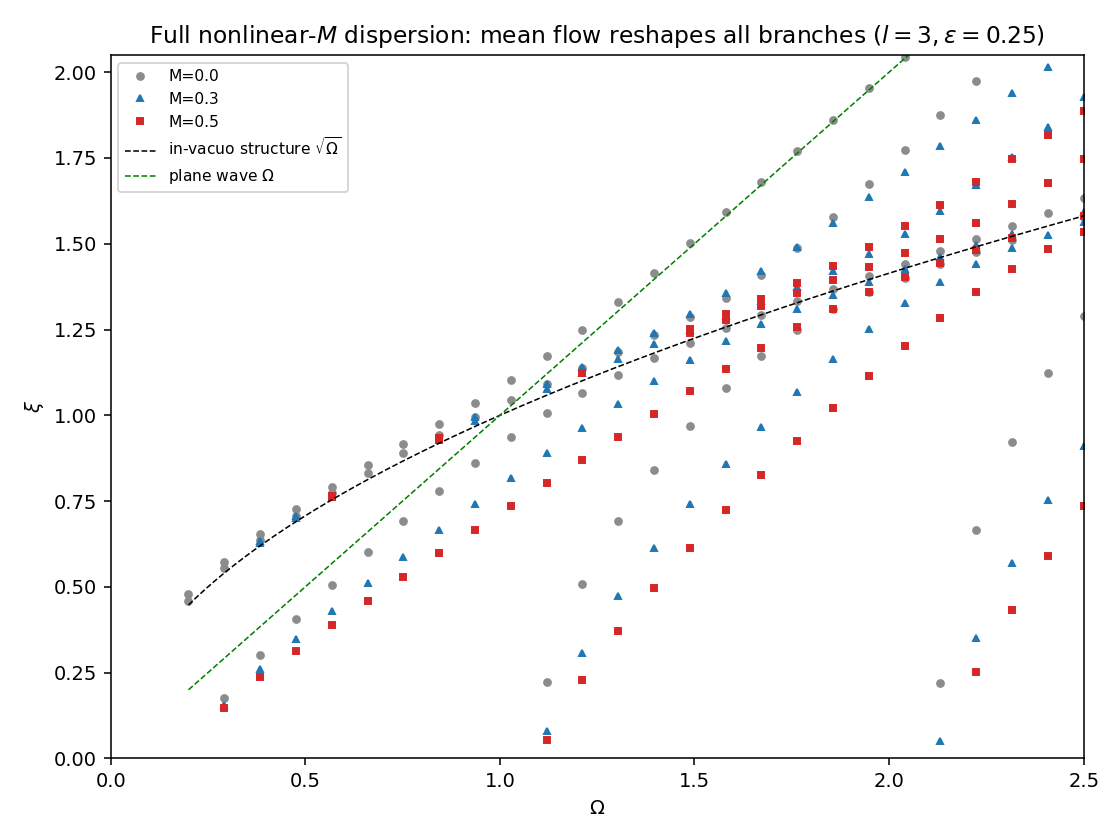
\includegraphics[width=0.72\textwidth]{fig9_Mmap.png}
\caption{Full nonlinear-in-$M$ dispersion ($l=3$, $\eps=0.25$): mean flow shifts every coupled branch
to lower $\xi$ with increasing downstream Mach number, most strongly near the plane wave.}
\label{fig:Mmap}
\end{figure}

\begin{figure}[h]
\centering
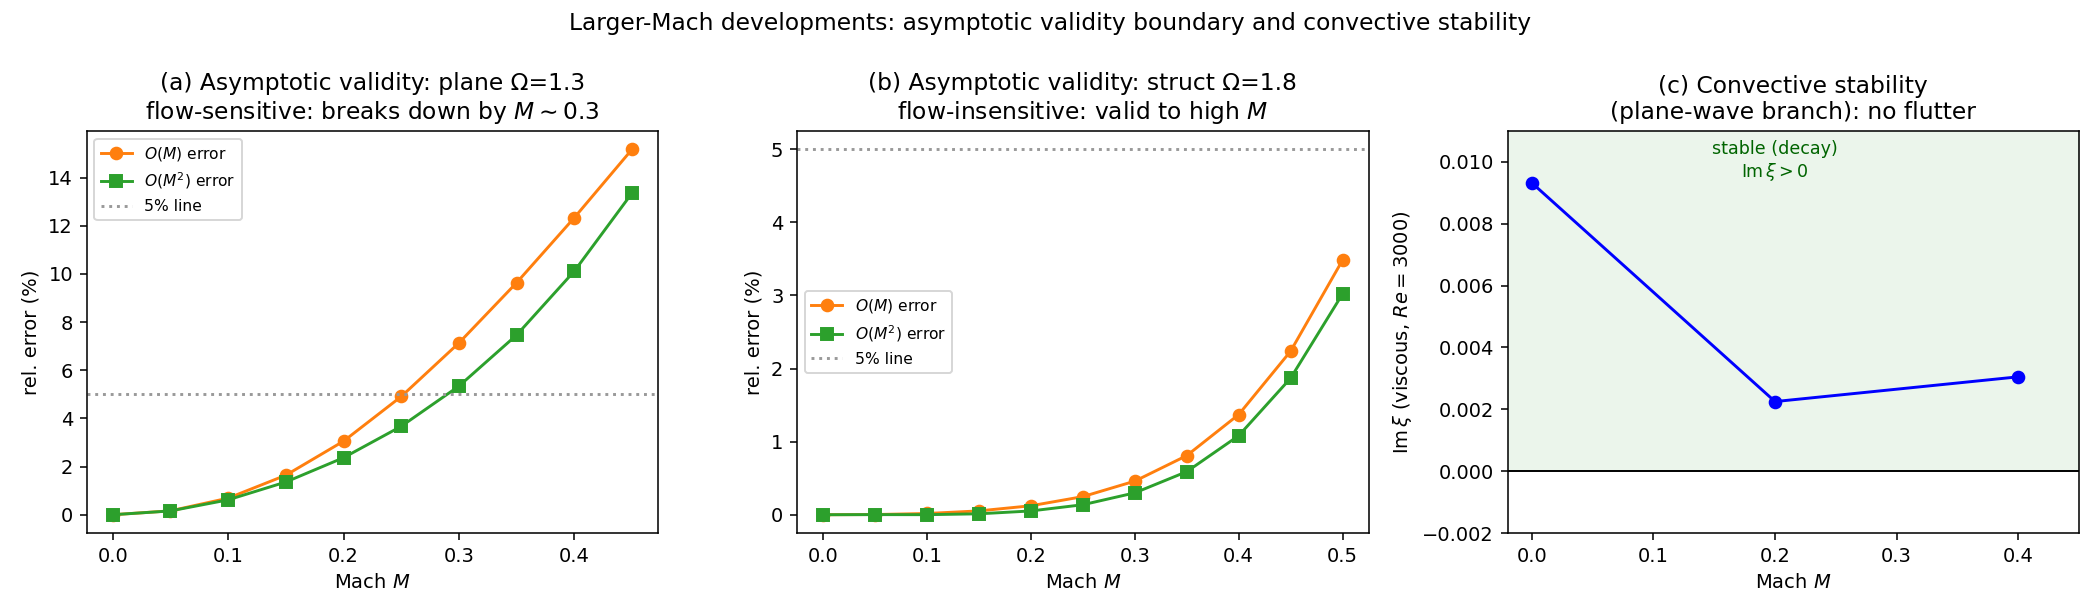
\includegraphics[width=0.99\textwidth]{fig10_validity_stability.png}
\caption{(a,b) Branch-dependent validity of the $O(M)$/$O(M^2)$ asymptotics: the flow-sensitive
plane-wave branch breaks down by $M\sim0.3$, while a flow-insensitive structural branch stays accurate
to larger $M$. (c) Convective stability: the viscous decay rate $\operatorname{Im}\xi>0$ (no flutter).}
\label{fig:valid}
\end{figure}

\section{Conclusions}
This paper has derived, and checked numerically, closed-form asymptotic expressions for the coupled
wavenumbers of a fluid column bounded by two flexible plates. The treatment generalises the work of
Sarkar and Sonti, and of Fahy, to both symmetry families and to non-identical plates, and it then goes
beyond the quiescent problem by admitting a low-Mach Poiseuille flow through the Pridmore--Brown
equation, for which a closed-form $O(M)$ correction, its $O(M^2)$ convection/shear refinement, and a
critical-layer analysis have all been worked out. Retaining viscosity shows that the eigenvalue stays
regular above $M_{\rm crit}$ and that the discrete wall modes are not absorbed by the critical layer,
their decay being controlled by the wall Stokes layers, scaling as $Re^{-1/2}$ and vanishing as the
viscosity is removed. Three independent numerical methods support the analysis throughout. The framework
is straightforward to implement with a symbolic-algebra package and keeps the physics transparent, and
the resulting expressions are of the kind a designer of a compliant duct or a flow-bearing elastic
waveguide could use directly. Two questions are left open for later work: the nonlinear,
finite-amplitude critical layer, and the contribution of the continuous spectrum.


\appendix
\section{Plate-admittance boundary conditions}\label{app:bc}
This appendix sets out the wall conditions used with the Pridmore--Brown equation~\eqref{eq:pb} in both
the inviscid and the viscous formulations, and shows that the two are consistent. Fields are taken to
vary as $e^{\mathrm{i}(\omega t-k_xx)}$, so that the material derivative becomes
$\mathrm{D}/\mathrm{D}t=\partial_t+U\partial_x\to\mathrm{i}(\omega-k_xU)=\mathrm{i}\sigma$. The essential
point is that the Poiseuille profile is no-slip: because $U(0)=U(a)=0$, at each wall $\sigma$ returns to
$\omega$ and the material derivative reduces to $\partial_t$, so that the convective (Ingard--Myers)
slip correction makes no contribution there.

\paragraph{Kinematic and plate-dynamic conditions.} Continuity of normal velocity gives
$v=\mathrm{D}w_j/\mathrm{D}t$, which at the walls, where $U=0$, is simply $v=\mathrm{i}\omega w_j$. The
plates obey $G_jw_j=\mp p$, with the minus sign at $y=0$, where the fluid lies above plate~1, and the
plus sign at $y=a$, where it lies below plate~2, and with $G_j=D_jk_x^4-m_j\omega^2$. Eliminating $w_j$
between these two statements gives
\begin{equation}
v(0)=-\frac{\mathrm{i}\omega}{G_1}\,p(0),\qquad v(a)=+\frac{\mathrm{i}\omega}{G_2}\,p(a).
\label{eq:adm}
\end{equation}

\paragraph{Inviscid form (used in \eqref{eq:pb}).} The inviscid $y$-momentum equation
$\rho\,\mathrm{D}v/\mathrm{D}t=-\partial_yp$ gives $v=\mathrm{i}\,p_y/(\sigma\rho)$, so that at $y=0$,
where $\sigma=\omega$, one has $v(0)=\mathrm{i}\,p_y(0)/(\omega\rho)$. Equating this to~\eqref{eq:adm}
yields $p_y(0)=-\omega^2\rho\,p(0)/G_1$, and non-dimensionalising with $\hat p=p/\rho c^2$, $\eta=y/a$,
$G_1=m_1\omega^2S_1$ and $\varepsilon=\rho a/m_1$ produces
\begin{equation}
\hat p_\eta(0)+\frac{\varepsilon}{S_1}\hat p(0)=0,\qquad
\hat p_\eta(1)-\frac{\varepsilon}{S_2}\hat p(1)=0,
\label{eq:robinp}
\end{equation}
which are the plate-admittance (Robin) conditions placed on the Pridmore--Brown pressure.

\paragraph{Viscous form (linearised Navier--Stokes, \S4.3).} Once viscosity is retained the velocity is
no longer slaved to $p_y$, and the pressure is instead recovered from the (inviscid-energy) continuity
relation $\mathrm{i}\sigma\,p+\rho c^2(-\mathrm{i}k_xu+\partial_yv)=0$, that is, in non-dimensional form,
$\hat p=\xi\hat u/\hat\sigma+\mathrm{i}\hat v_\eta/(l\hat\sigma)$. Imposing no-slip, $\hat u=0$, at the
wall, where $\hat\sigma=\Omega$, gives $\hat p(0)=\mathrm{i}\hat v_\eta(0)/(l\Omega)$. Substituting this
into the non-dimensional admittance~\eqref{eq:adm}, $\hat v(0)=-\mathrm{i}\varepsilon\hat p(0)/(l\Omega
S_1)$, turns the condition into a Robin condition on the normal velocity,
\begin{equation}
\hat v(0)-\beta_1\hat v_\eta(0)=0,\qquad \hat v(1)+\beta_2\hat v_\eta(1)=0,\qquad
\beta_j=\frac{\varepsilon}{l^2\Omega^2S_j}.
\label{eq:robinv}
\end{equation}
As $Re\to\infty$ the viscous $y$-momentum balance returns to its inviscid form and~\eqref{eq:robinv}
returns to~\eqref{eq:robinp}; both reductions, and the coefficients $\beta_j$ themselves, were checked
symbolically. Together, the no-slip condition $\hat u=0$ and~\eqref{eq:robinv} supply the four boundary
conditions that the fourth-order viscous system requires.
\begin{thebibliography}{9}
\bibitem{sarkarsonti} A.\ Sarkar, V.R.\ Sonti, An asymptotic analysis for the coupled dispersion
characteristics of a structural acoustic waveguide, \emph{J.\ Sound Vib.}\ \textbf{306} (2007) 657--674.
\bibitem{fahy} F.\ Fahy, \emph{Sound and Structural Vibration: Radiation, Transmission and Response},
Academic Press, 1989, pp.\ 259--268, 136--140.
\bibitem{kunte2011} A.\ Sarkar, M.V.\ Kunte, V.R.\ Sonti, Unified dispersion characteristics of
structural acoustic waveguides, \emph{Comput.\ Model.\ Eng.\ Sci.}\ \textbf{81} (3\&4) (2011) 249--268.
\bibitem{prakash2016} V.\ Prakash, V.R.\ Sonti, A systematic asymptotic approach to determine the
dispersion characteristics of structural-acoustic waveguides with arbitrary fluid loading,
\emph{J.\ Sound Vib.}\ \textbf{373} (2016) 164--179.
\bibitem{morseingard} P.M.\ Morse, K.U.\ Ingard, \emph{Theoretical Acoustics}, McGraw--Hill, 1968,
pp.\ 624--634.
\bibitem{crighton} D.G.\ Crighton, The 1988 Rayleigh Medal Lecture: fluid loading---the interaction
between sound and vibration, \emph{J.\ Sound Vib.}\ \textbf{133} (1) (1989) 1--27.
\bibitem{pridmorebrown} D.C.\ Pridmore-Brown, Sound propagation in a fluid flowing through an
attenuating duct, \emph{J.\ Fluid Mech.}\ \textbf{4} (1958) 393--406.
\bibitem{brambley} E.J.\ Brambley, A well-posed boundary condition for acoustic liners in straight
ducts with flow, \emph{AIAA J.}\ \textbf{49} (6) (2011) 1272--1282.
\bibitem{brambleydarau} E.J.\ Brambley, M.\ Darau, S.W.\ Rienstra, The critical layer in linear-shear
boundary layers over acoustic linings, \emph{J.\ Fluid Mech.}\ \textbf{710} (2012) 545--568.
\bibitem{maslowe} S.A.\ Maslowe, Critical layers in shear flows, \emph{Annu.\ Rev.\ Fluid Mech.}\
\textbf{18} (1986) 405--432.
\bibitem{morab} S.R.\ Morab, A.\ Sharma, J.S.\ Murallidharan, Low Mach number approximated linearized
perturbed Euler equations-based unified computational flow-induced acoustic model for 2D
planar/axisymmetric complex geometry, \emph{J.\ Comput.\ Phys.}\ \textbf{514} (2024) 113242.
\end{thebibliography}

\end{document}
